\svnid{$Id$}

\section{Additive Schwarz methods}

\begin{intro}
  In this section, we study preconditioners, which are related to
  subspace decompositions of the space $V$ or its finite dimensional
  subspaces. We will develop the theory in an abstract way, but always
  keep the model problem~\eqref{eq:itintro:1} in mind when we do so. In
  particular, the subspaces chosen will be associated with either
  coarser mesh levels or with meshes on subdomains of $\Omega$.
  
  This section follows in part~\cite[Chapter 7]{BrennerScott02}. A
  more detailed discussion with extension of the methods developed
  here can be found in~\cite{ToselliWidlund05}
\end{intro}

\subsection{The abstract framework}

\begin{intro}
  Let $V$ be a Hilbert space and let $a(.,.): V\times V$ be a
  symmetric and $V$-elliptic bilinear form. Let the set of auxiliary
  subspaces $\{V_j\}_{j=1,\dots,J}$ of $V$ be chosen such that
  \begin{gather*}
    V = \sum_{j=1}^J V_j,
  \end{gather*}
  but the sum is not required to be direct, that is, a vector $v\in V$
  may have several decompositions $v = \sum \alpha_j v_j$ with $v_j\in
  V_j$.
\end{intro}

\begin{lemma}
  \label{lemma:schwarz:1}
  If the form $a(.,.)$ is bounded and V-elliptic, then the weak
  formulation: find $u_j\in V_j$ such that
  \begin{gather}
    \label{eq:schwarz:1}
    a(u_j,v_j) = f(v_j),
    \quad\forall v_j\in V_j,
  \end{gather}
  has a unique solution for all $f\in V^*$.
\end{lemma}

\begin{proof}
  This lemma follows from the fact that boundedness and V-ellipticity
  transfer from $V$ to its subspaces.
\end{proof}

\begin{definition}
  \label{definition:schwarz:1}
  \index{Pj@$P_j$}
  Let the operator $P_j: V \to V_j$ be defined as the solution
  operator $P_j u := u_j$ to the problem
  \begin{gather}
    \label{eq:schwarz:2}
    a(u_j,v_j) = a(u,v_j),\quad\forall v_j\in V_j.
  \end{gather}
  \index{A-orthogonal projection@$A$-orthogonal projection}
  We call $P_j$ the $A$-orthogonal projection or \define{Ritz-projection} to
  $V_j$. The left hand side of this equation induces an operator $A_j:
  V_j \to V_j^*$ by $A_j u_j = a(u_j,.)$.

 Furthermore, we define the $V$-orthogonal projection operator
  \index{Pij@$\Pi_j$}
  $\Pi_j: V \to V_j$ as the solution operator $\Pi_j u := u_j$ to the problem
  \begin{gather}
    \label{eq:schwarz:3}
    \scal(u_j,v_j) = \scal(u,v_j),\quad\forall v_j\in V_j.
  \end{gather}
\end{definition}

\begin{lemma}
  \label{lemma:schwarz:2}  
  From definition~\ref{definition:schwarz:1}, we deduce
  \begin{gather}
    \label{eq:schwarz:15}
    A_j P_j = \Pi_j A.
  \end{gather}
\end{lemma}

\begin{proof}
  We rewrite equation~\eqref{eq:schwarz:2} as
  \begin{gather}
    \scal(A_j P_j u, v_j) = \scal(A u, v_j) = \scal(\Pi_j A u, v_j).
  \end{gather}
\end{proof}

\begin{definition}
  The additive Schwarz preconditioner for the operator $A$ associated
  with the symmetric, and $V$-elliptic bilinear form $a(.,.)$ with
  respect to the subspace decomposition $V_j$ is the mapping $B:
  V \to V^*$ such that
  \begin{gather}
    \label{eq:schwarz:4}
    B^{-1} = \sum_{j=1}^J P_j A^{-1}.
  \end{gather}
\end{definition}

\begin{example}
  The Jacobi iteration may serve as a guiding example for the
  definition of these methods. To this end, let $V = \R^n$ with its
  Euclidean inner product $\scal(.,.)$. let $V_j =
  \operatorname{span}\{e_j\}$ be the space spanned by the $j$th unit
  vector. Let $A$ be a symmetric, positive definite matrix and $a(u,v)
  = v^T A u$. Then, equation~\eqref{eq:schwarz:2} becomes
  \begin{gather*}
    e_j^T A u_j = e_j^T A u
    \quad \Leftrightarrow \quad
    P_j u = u_j = \frac1{a_{j j}}(A u)_j.
  \end{gather*}
  Since for this decomposition, the sum $V=\bigoplus V_j$ is direct,
  we obtain with $D=\operatorname{diag}(a_{11},\dots,a_{n n})$ the
  matrix representation
  \begin{gather*}
    (B^{-1} u)_j = \frac1{a_{j j}}(A A^{-1} u)_j
    \quad \Leftrightarrow \quad
    B^{-1} = D^{-1}.
  \end{gather*}
  From the Richardson method in operator
  form~\eqref{eq:richardson:11}, we obtain the iteration
  \begin{align*}
    u^{(k+1)} &= u^{(k)} - \omega_k \sum_{j=1}^J P_j \bigl(u^{(k)} -
    A^{-1}f\bigr)\\
    &= u^{(k)} - \omega_k D^{-1} \bigl(A u^{(k)} - f\bigr).
  \end{align*}
\end{example}

\begin{lemma}
  \label{lemma:schwarz:3}
  If $A$ is symmetric and positive definite, so is $B^{-1}$ as defined
  in~\eqref{eq:schwarz:4}.
\end{lemma}

\begin{proof}
  By Lemma~\ref{lemma:schwarz:2} and the fact that $P_j$ maps into $V_j$, we have that
  \begin{gather}
    \label{eq:schwarz:16}
    B^{-1} = \sum_{j=1}^J A_j^{-1} \Pi_j.
  \end{gather}
  Due to equation~\eqref{eq:schwarz:1}, $A_j$ inherits its symmetry
  and positive definiteness from $A$, and thus $A_j^{-1}$ is s.p.d.
  Therefore, for each term in this sum, we have
  \begin{gather*}
    \scal(A_j^{-1} \Pi_j u, v)
    = \scal(A_j^{-1} \Pi_j u, \Pi_j v)
    = \scal( \Pi_j u, A_j^{-1}\Pi_j v)
    = \scal(u, A_j^{-1}\Pi_j v).
  \end{gather*}
  The result now follows by linearity.
\end{proof}

\begin{lemma}
  \label{lemma:schwarz:5}
  For $v\in V$ holds
  \begin{gather}
    \label{eq:schwarz:5}
    b(v,v) \equiv \scal(B v,v) = \min_{v=\sum v_j} \sum_{j=1}^J a(v_j,v_j),
  \end{gather}
  where the minimum is taken over all possible decompositions of $v$
  into a sum of elements $v_j\in V_j$ with $j=1,\dots,J$.
\end{lemma}

\begin{proof}
  Since $B^{-1}$ is s.p.d., so is $B$. Therefore, $\scal(.,A_j^{-1}.)$
  is an inner product on $V_j^*$, for which the Bunyakovsky-Cauchy-Schwarz
  inequality holds. Thus, for an arbitrary decomposition $v=\sum v_j$
  with $v_j\in V_j$, the computation
  \begin{align*}
    b(v,v)
    &= \sum_{j=1}^J b(v, A_j^{-1} A_j v_j)
    = \sum_{j=1}^J \scal(\Pi_j B v, A_j^{-1} A_j v_j) \\
    &\le \sum_{j=1}^J \sqrt{\scal(\Pi_j B v, A_j^{-1}\Pi_j B v)}
    \sqrt{\scal(A_j v_j, A_j^{-1}A_j v_j)} \\
    & \le \sqrt{\sum_{j=1}^J \scal(\Pi_j B v, A_j^{-1}\Pi_j
      B v) }
    \sqrt{\sum_{j=1}^J \scal(A_j v_j,A_j^{-1}A_j v_j)} \\
    &= \sqrt{\scal(B v, {\sum A_j^{-1}\Pi_j} B v)}
    \sqrt{\sum_{j=1}^J \scal(A_j v_j, v_j)} \\
    &= \sqrt{b(v,v)} \sqrt{\sum_{j=1}^J a(v_j, v_j)},
  \end{align*}
  yields for arbitrary decompositions
  \begin{gather}
    \label{eq:schwarz:17}
    b(v,v) \le \sum_{j=1}^J a(v_j, v_j),
  \end{gather}
  and thus in particular, that the left hand side is bounded by the
  minimum of the right. Now we choose a special decomposition, showing
  that it cannot be less than the minimum. To this end, let
  \begin{gather}
    \label{eq:schwarz:18}
    v_j = A_j^{-1} \Pi_j B v.
  \end{gather}
  By Lemma~\ref{lemma:schwarz:2}, we have
  \begin{gather*}
    \sum v_j = \sum A_j^{-1} \Pi_j B v = B^{-1} B v = v.
  \end{gather*}
  Furthermore,
  \begin{align*}
    \sum_{j=1}^J \scal(A_j v_j, v_j)
    &= \sum_{j=1}^J \scal(A_j A_j^{-1} \Pi_j B v, A_j^{-1} \Pi_j
    B v) \\
    &= \sum_{j=1}^J \scal(\Pi_j B v, A_j^{-1} \Pi_j v) \\
    &= \scal(B v, \sum A_j^{-1} \Pi_j B v) = b(v, v).
  \end{align*}
\end{proof}

\begin{theorem}
  \label{theorem:schwarz:1}
  Let $A$ be s.p.d. and $B$ defined by
  equation~\eqref{eq:schwarz:4}. Then, the \putindex{spectral
    equivalence}~\eqref{eq:richardson:12} holds with
  positive constants
  \begin{gather}
    \label{eq:schwarz:19}
%    \begin{split}
    \Lambda(B,A) = \max_{v\in V} \frac{a(v,v)}{\min\limits_{v=\sum v_j}
      \sum\limits_{j=1}^J a(v_j, v_j)}
    ,\qquad
    \lambda(B,A) = \min\limits_{v\in V} \frac{a(v,v)}{\min\limits_{v=\sum v_j}
      \sum\limits_{j=1}^J a(v_j, v_j)}.
%    \end{split}
  \end{gather}
\end{theorem}

\begin{proof}
  Here we use the fact, that $b(.,.)$ is an inner product on
  $V$ and that by
  \begin{gather*}
    b(B^{-1}A v,v) = a(v,v) = b(v, B^{-1}A v),
  \end{gather*}
  the operator $B^{-1}A$ is symmetric with respect to this inner
  product. Thus, the \putindex{Rayleigh quotient} qualifies to
  estimate the extremal eigenvalues, for instance,
  \begin{gather*}
    \Lambda(B^{-1}A)
    = \max_{v\in V} \frac{b(B^{-1}A v,v)}{b(v,v)}
    = \max_{v\in V} \frac{a(v,v)}{\min\limits_{v=\sum v_j}
      \sum\limits_{j=1}^J a(v_j, v_j)},
  \end{gather*}
  and the same for the minimum.
\end{proof}

\begin{note}
  \label{note:schwarz:1}
  In order to estimate the condition number $\Lambda(B,A)/\lambda(B,A)$ of a Schwarz
  preconditioner, it is now sufficient to bound the two quotients
  in~\eqref{eq:schwarz:19} from above and below. In particular, in
  order to find a bound for $\Lambda(B,A)$, we have to find an estimate of
  the form
  \begin{gather}
    \label{eq:schwarz:23}
    a(v,v) \lesssim \min_{v=\sum v_j}\sum_{j=1}^J a(v_j, v_j),
  \end{gather}
  or in other words, $a(v,v)$ has to be bounded by the sum on the
  right for any decomposition $v=\sum v_j$. On the other hand, in
  order to bound $1/\lambda(B,A)$, we need an estimate of the form
  \begin{gather}
    \label{eq:schwarz:24}
     \min_{v=\sum v_j}\sum_{j=1}^J a(v_j, v_j) \lesssim a(v,v),
  \end{gather}
  where it is sufficient to find one decomposition $v=\sum v_j$ such
  that the sum is bounded by the right hand side.
\end{note}

%%%%%%%%%%%%%%%%%%%%%%%%%%%%%%%%%%%%%%%%%%%%%%%%%%%%%%%%%%%%%%%%%%%%%%
%%%%%%%%%%%%%%%%%%%%%%%%%%%%%%%%%%%%%%%%%%%%%%%%%%%%%%%%%%%%%%%%%%%%%%
\section{Two-level additive Schwarz preconditioner}
%%%%%%%%%%%%%%%%%%%%%%%%%%%%%%%%%%%%%%%%%%%%%%%%%%%%%%%%%%%%%%%%%%%%%%
%%%%%%%%%%%%%%%%%%%%%%%%%%%%%%%%%%%%%%%%%%%%%%%%%%%%%%%%%%%%%%%%%%%%%%

\begin{intro}
  This preconditioner is in the class of \putindex{domain
    decomposition} methods. The attribute \putindex{two-level} refers
  to the fact that we are considering finite element discretizations
  of~\eqref{eq:itintro:1} on two finite element meshes, the
  \putindex{fine mesh} $\T_h$ on which we desire to compute the
  solution, and the auxiliary \putindex{coarse mesh} $\T_H$. Both
  meshes cover the whole domain $\Omega$ (see
  Figure~\ref{fig:schwarz:ddmeshes}), and each cell of the coarse mesh
  is the union of cells of the fine mesh ($4\times 4$ fine cells in
  the figure).

  In addition to these two meshes, we introduce subdomains
  $\Omega_1,\Omega_2,\dots,\Omega_J$ of $\Omega$ such that each
  $\Omega_j$ is the union of cells in $\T_h$. We require that those
  subdomains overlap each other like the three examples in
  Figure~\ref{fig:schwarz:ddmeshes} on the right. A more precise
  definition of the required overlap follows.

  \index{NO@$N_O$}
  Furthermore, we assume that there is a constant $N_O$ independent of
  $\T_h$ and the number of subdomains, such that for each $j$ the
  intersection $\Omega_j\cap\Omega_k$ is nonempty for at most $N_O$
  subdomains $\Omega_k$.
\end{intro}

\begin{figure}[tp]
  \centering
  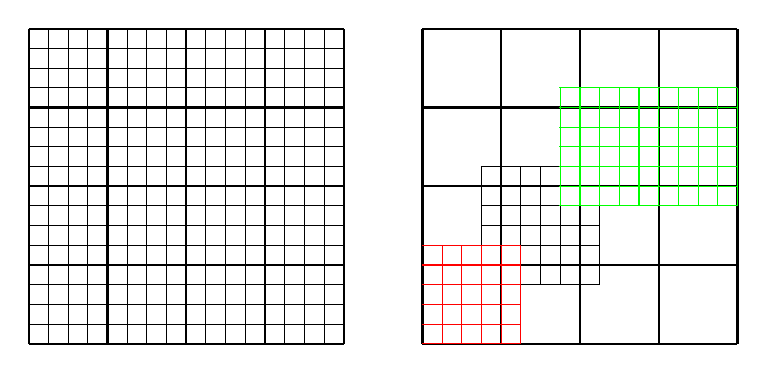
\begin{tikzpicture}
    \draw[step=.25cm] (-2,-2) grid (2,2);
    \draw[step=1cm,thick] (-2,-2) grid (2,2);
    \draw[step=1cm,thick] (3,-2) grid (7,2);
    \draw[step=.25cm] (3.74,-1.25) grid (5.25,0.25);
    \draw[step=.25cm,red] (3,-2) grid (4.25,-0.75);
    \draw[step=.25cm,green] (4.74,-0.25) grid (7,1.25);
  \end{tikzpicture}
  \caption{Fine mesh and coarse mesh (left) for overlapping domain
    decomposition. Examples for a subdomain decomposition on the
    right.}
  \label{fig:schwarz:ddmeshes}
\end{figure}

\begin{definition}
  A covering of $\Omega$ with subdomains $\Omega_j$ is called
  \define{overlapping} with minimal \define{overlap} $\delta$, if for
  each $\Omega_j$ and all $x\in\Omega_j$ holds:
  \begin{gather*}
    \operatorname{dist}(x,\partial\Omega_J\setminus\partial\Omega) <
    \delta\;
    \Rightarrow\; \exists k\neq j: x\in \Omega_k.
  \end{gather*}
\end{definition}

\begin{definition}
  A smooth \define{partition of unity} with respect to the subdomains
  $\Omega_1,\Omega_2,\dots,\Omega_J$ of $\Omega$ is a set of
  nonnegative functions $\{\phi_1,\dots,\phi_J\}\subset
  C^\infty(\overline\Omega)$ such that
  \begin{xalignat}2
    \label{eq:schwarz:6}
    \phi_j(x) &  = 0
    & \forall x & \in \Omega\setminus\Omega_j, \quad j=1,\dots,J
    \\
    \label{eq:schwarz:7}
    \sum_{j=1}^J \phi_j(x) &= 1
    & \forall x&\in\overline\Omega.
  \end{xalignat}
  Similarly, we can define partitions of unity in $H^1(\Omega)$ or
  partitions of unity which are piecewise $C^1$.
  
  Furthermore, we assume that there is a positive constant $\delta$,
  called \define{overlap}, such that for all $j=1,\dots,J$ there holds
  \begin{gather}
    \label{eq:schwarz:8}
    \norm{\nabla\phi j}_{L^\infty(\Omega)} \lesssim \frac 1\delta,
  \end{gather}
  where the implicit constant is independent of $h$, $\delta$ and $J$.
\end{definition}

\begin{note}
  The term overlap for $\delta$ is justified by the following
  consideration. Let $x \in \Omega_j$ be a point which is not in any
  other $\Omega_i$. Then, $\phi_j(x) = 1$. If~\eqref{eq:schwarz:8} is
  to hold, then it is necessary that
  $\operatorname{dist}(x,\partial\Omega_J) \ge \delta$ (up to a
  constant, but this constant is already
  in~\eqref{eq:schwarz:8}). Thus, the points of distance less than
  $\delta$ from $\partial\Omega_j$ must be elements of another
  subdomain as well, which is then said to overlap with $\Omega_j$.
\end{note}

\begin{example}
  \label{example:schwarz:2}
  On uniform meshes, overlapping subdomains with an overlap of
  $\delta = n h$ with $n=1,2,\ldots$ can be achieved easily by the
  following procedure:
  \begin{enumerate}
  \item Begin with a non overlapping subdivision $\{\Omega_j^0\}$,
    for instance aligned with the mesh cells of $\T_H$.
  \item Add all cells that share at least a vertex with a cell in
    $\Omega_j^0$ to obtain a domain $\Omega_j^1$. After this
    procedure, two neighboring domains will overlap by two cells,
    resulting in $\delta = 2h$.
  \item Repeat this procedure to obtain larger overlaps.
  \end{enumerate}
  
  On the resulting partitions, a partition of unity in $H^1$ can be
  constructed with piecewise linear (bilinear on quadrilaterals)
  functions. For instance for $\Omega_j^1$ this function is
  constructed as follows:
  \begin{enumerate}
  \item Choose $\phi_j(x) = 1/2$ in all vertices on $\partial \Omega_j^0$.
  \item Choose $\phi_j(x) = 0$ in all vertices on $\partial \Omega_j^1$ and outside
    $\Omega_j^1$.
  \item Choose $\phi_j(x) = 1$ in all remaining vertices inside
    $\Omega_j^0$.
    \item Connect these values by linear (on simplicial meshes), bilinear
      (quadrilateral meshes) of trilinear (hexahedral meshes)
      polynomials inside each mesh cell $T\in \T_h$.
  \end{enumerate}
  This partition of unity achieves the estimate~\eqref{eq:schwarz:8}
  with a constant of $1/2$.
\end{example}

\begin{notation}
  The solution space of our problem is the space $V=V_h$ given by the
  finite element space on the mesh $\T_h$. We define finite element
  spaces on $\Omega_j$ by
  \begin{gather}
    \label{eq:schwarz:9}
    V_j = \bigl\{ v\in V_h \big| \forall x\in\Omega\setminus\Omega_j :
    v(x) =0\bigr\}.
  \end{gather}
  Additionally, we define the space $V_0 \equiv V_H$ as the finite
  element space on the coarse mesh $\T_H$.  Since the meshes are
  nested, $V_H$ is indeed a subspace of $V_h$. Thus, we obtain a
  decomposition of $V_h$ into $J+1$ subspaces
  \begin{gather*}
    V_h = V_0 + \sum_{j=1}^J V_j,
  \end{gather*}
  where the last $J$ are associated with the subdomains. In fact,
  Lemma~\ref{lemma:schwarz:4} below states that already the spaces
  $V_1$ to $V_J$ are sufficient to span $V_h$. Nevertheless, the
  coarse grid space plays a crucial role in the efficiency of the
  method due to Lemma~\ref{lemma:schwarz:stable-decomposition}.
\end{notation}

\begin{definition}
  Let the spaces $V_j$, $j=0,\dots,J$ be defined as above. Then, the
  \define{two-level additive Schwarz preconditioner} is defined as
  \begin{gather}
    \label{eq:schwarz:10}
    B^{-1}_{\text{TLS}} = \sum_{j=0}^J P_j A^{-1} = \sum_{j=0}^J A_j^{-1} \Pi_j,
  \end{gather}
  where $P_j$ is defined according to~\eqref{eq:schwarz:2} and $A_j:
  V_j\to V_j^*$ by
  \begin{gather}
    \scal(A_j u_j, v_j)_V = a(u_j, v_j),\quad\forall u_j, v_j \in V_j.
  \end{gather}
\end{definition}

\begin{note}
  In order to simplify notation, we have assigned index zero to
  $V_H$. Thus, sums in future terms may either start at one, summing
  over subdomains, or at zero, summing over all subspaces.
\end{note}

\begin{lemma}
  \label{lemma:schwarz:4}
  There holds
  \begin{gather}
    \label{eq:schwarz:11}
    V_h = \sum_{j=1}^J V_j.
  \end{gather}
\end{lemma}

\begin{proof}
  Let $I_h: C(\overline\Omega) \to V_h$ be the interpolation operator
  of the finite element space. Then, for any given $v\in V_h$ define
  $v_j = I_h(\phi_j v)$, where $\phi_j$ is the function associated to
  $\Omega_j$ of a partition of unity for $\Omega_1,\dots,\Omega_J$.
  
  By definition of $\phi_j$, there holds $\phi_j v = 0$ on
  $\Omega\setminus\Omega_j$. Furthermore, we assumed that a mesh cell
  of $\T_h$ is either completely in $\Omega_j$ or completely in its
  complement. Since nodal values of a cell are located in the cell
  itself, this implies that $I_h (\phi_j v) = 0$ on
  $\Omega\setminus\Omega_j$. Therefore, $I_h (\phi_j v) \in V_j$.
  
  On the other hand, we use the linearity of the interpolation
  operator to obtain
  \begin{gather*}
    \sum_{j=1}^J v_j = \sum_{j=1}^J I_h(\phi_j v)
    = I_h\left(v\sum_{j=1}^J \phi_h\right)
    = I_h v = v,
  \end{gather*}
  thus, the $v_j$ are indeed a decomposition of $v$. Since $v\in V_h$
  was chosen arbitrarily, the lemma is proven.
\end{proof}

\begin{lemma}
  \label{lemma:schwarz:6}
  Let $v_j\in V_j$ for $j=0,\dots,J$ be a composition of $v\in V_h$
  such that
  \begin{gather*}
    v=\sum_{j=0}^J v_j.
  \end{gather*}
  Then,
  \begin{gather}
    \label{eq:schwarz:12}
    a(v,v) \lesssim \sum_{j=0}^J a(v_j, v_j),
  \end{gather}
  where the implicit constant does not depend on $h$, $H$, or $J$.
\end{lemma}

\begin{proof}
  First a note: the inequality would be obvious, if $V_h$ was a direct
  sum of the spaces $V_j$, and it would hold with a constant of one if
  they were mutually orthogonal. Thus, we have to show some kind of
  orthogonality between the spaces.

  We start out by stating that
  \begin{align*}
    a(v,v) &= a\left(v_0+\sum_{j=1}^J v_j, v_0+\sum_{j=1}^J v_j\right)
    \\
    &\le 2 \left(a(v_0, v_0) + a\!\left(\sum_{j=1}^J v_j,\sum_{j=1}^J
        v_j\right)\right)
    \\
    &= 2 \left(a(v_0, v_0) + 2 \sum_{j,k=1}^J a(v_j,v_k)\right).
  \end{align*}

  In order to estimate the second term on the right, we observe that
  $a(v_j,v_k)\neq 0$ only if $\Omega_j$ and $\Omega_k$ overlap (this
  is as much orthogonality as we get). Let therefore $o_{j k}$ be a
  coefficient such that
  \begin{gather*}
    o_{j k} =
    \begin{cases}
      1 & \Omega_j \cap \Omega_k \neq \emptyset \\
      0 & \Omega_j \cap \Omega_k = \emptyset
    \end{cases}
  \end{gather*}
  Now we obtain
  \begin{align*}
    \sum_{j,k=1}^J a(v_j,v_k)
    &= \sum_{j,k=1}^J o_{j k}  a(v_j,v_k) \\
    & \le \sum_{j,k=1}^J \sqrt{o_{j k} a(v_j, v_j)} \sqrt{o_{j k} a(v_k,
      v_k)} \\
    & \le \sum_{j,k=1}^J o_{j k} a(v_j, v_j) \\
    & \le N_O \sum_{j=1}^J a(v_j, v_j).
  \end{align*}
\end{proof}


\begin{lemma}[Stable decomposition]
  \label{lemma:schwarz:stable-decomposition}
  For each $v\in V_h$ there exists a decomposition $v=\sum_{j=0}^J
  v_j$ with $v_j\in V_j$, such that
  \begin{gather}
    \label{eq:schwarz:13}
    \sum_{j=0}^J a(v_j, v_j)
    \lesssim \left(1+\frac H\delta\right)^2 a(v,v).
  \end{gather}
\end{lemma}

\begin{proof}
  Let $\tilde I_H: H^1_0(\Omega) \to V_H$ be an interpolation operator
  continuous on $H^1(\Omega)$, for instance the interpolation operator
  by Clement or the one by Scott and Zhang. For a given function
  $v\in V_h$, let $v_H = \tilde I_H v$. Then
  \begin{gather}
    \label{eq:schwarz:20}
    \begin{split}
      |v_H|_1 &\lesssim |v|_1 \\
      \|v-v_H\|_0 &\lesssim H |v|_1.
    \end{split}
  \end{gather}
  From~\eqref{eq:schwarz:20} there holds
  \begin{gather}
    \label{eq:schwarz:22}
    a(v_H,v_H) = |v_H|_1^2 \lesssim |v|_1^2 = a(v,v).
  \end{gather}
  Let $w=v-v_H$. Using a partition of unity $\{\phi_j\}$ for the
  subdomains $\{\Omega_j\}$ and the nodal interpolant $I_h$ as in the
  proof of Lemma~\ref{lemma:schwarz:4}, and let
  \begin{gather*}
    v_j = I_h(\phi_j w).
  \end{gather*}
  Thus, $v = \sum v_j$. We point out, that we can use the nodal
  interpolant, since $w$ is a finite element function on $\T_h$ and
  $\phi_j$ is either smooth or piecewise polynomial. For the remainder
  of this proof, we will assume the piecewise polynomial case (see
  Example~\ref{example:schwarz:2}) and leave the arguments for a
  smooth function $\phi_j$ to the reader.
  
  The interpolation operator is exact for polynomials of degree $k$
  (assuming such an order for the finite element being
  used). Therefore,
  \begin{gather*}
    a(v_j,v_j) = |v_j|_1^2 \lesssim |\phi_j w|_1^2
    \lesssim \|\nabla \phi_j w\|_0^2 + \|\phi_j \nabla w\|_0^2.
  \end{gather*}
  Using the properties of the partition of unity, we obtain
  \begin{gather*}
    a(v_j,v_j) \lesssim \frac1{\delta^2} \|\chi(\Omega_j) w\|_0^2 + |\chi(\Omega_j)w|_1^2.
  \end{gather*}
  Summing up yields
  \begin{gather}
    \label{eq:schwarz:21}
    \begin{split}
      \sum_{j=1}^J a(v_j, v_j)
      &\lesssim \sum_{j=1}^J \left(\frac1{\delta^2} \|\chi(\Omega_j)
        w\|_0^2 + |\chi(\Omega_j)w|_1^2\right) \\
      &\le N_O \left(\frac1{\delta^2}\|w\|_0^2 + |w|_1^2\right) \\
      &=  N_O \left(\frac1{\delta^2} \|v-v_H\|_0^2 + |v-v_H|_1^2\right)
      \\
      & \lesssim \frac{H^2}{\delta^2} |v|_1^2 + |v|_1^2 \\
      &= \left(1+\frac{H^2}{\delta^2}\right) a(v,v).      
    \end{split}
  \end{gather}
  The estimate~\eqref{eq:schwarz:13} now follows
  from~\eqref{eq:schwarz:22} and~\eqref{eq:schwarz:21}.
\end{proof}

\begin{theorem}
  \label{theorem:schwarz:two-level-convergence}
  Under the assumptions made so far in this section, there holds
  \begin{gather}
    \label{eq:schwarz:14}
    \kappa(B^{-1}_{\text{TLS}} A_h)
    = \frac{\Lambda(B_{\text{TLS}}, A_h)}{\lambda(B_{\text{TLS}},
      A_h)}
    \lesssim \left(1+\frac H\delta\right)^2,
  \end{gather}
  where the implicit constant is independent of $h$, $\delta$, $H$, and $J$.
\end{theorem}

\begin{proof}
  The proof follows Note~\ref{note:schwarz:1}. Indeed,
  Lemma~\ref{lemma:schwarz:6} proves inequality~\eqref{eq:schwarz:23}
  and Lemma~\ref{lemma:schwarz:stable-decomposition}
  proves~\eqref{eq:schwarz:24}.
\end{proof}

\begin{remark}
  We have constructed a preconditioner $B_{\text{TLS}}$ for the finite
  element discretization of the Poisson problem~\eqref{eq:itintro:1}
  such that the preconditioned system has a bounded condition number
  independent of the mesh size $h$. Thus, a Richardson iteration or a
  conjugate gradient method using this preconditioner will reduce the
  error by a certain amount within a fixed number of steps.
  
  Closer inspection of the estimate~\eqref{eq:schwarz:14} in view of
  Example~\ref{example:schwarz:2} reveals a problem though: typically,
  $\delta$ is of the order of $h$, such that the estimate becomes
  \begin{gather*}
    \kappa(B^{-1}_{\text{TLS}} A_h) \lesssim \left(1+\frac H h\right)^2.
  \end{gather*}
  If we choose $H$ constant, this is exactly as bad as the condition
  number of $A$ itself. Under mild further assumptions, the square on
  the right hand side can be avoided~\cite{DryjaWidlund94}, which
  is an improvement compared to the operator without preconditioning,
  but is not uniform with respect to $h$. Therefore, we are left with
  two options:
  \begin{enumerate}
  \item Increase the overlap such that it is $\mathcal O(H)$. This
    procedure yields a \putindex{uniform preconditioner}, but it
    introduces a problem: when refining $h$, more and more
    cells belong to several subdomains and thus computations on them
    have to be performed several times. Therefore, the effort per
    preconditioning step is increased considerably.
  \item Keep the overlap at a small multiple of $h$ and choose $H$
    such that $H/h$ is bounded by a constant. Then, the preconditioner
    remains uniform, the overlap remains small. This way, the
    difficulty has been transferred to the coarse grid problem on
    $\T_H$, since now this problem becomes more and more difficult to
    solve, when $h$ decreases.
  \end{enumerate}
  
  While the problems of the first option above are inherent and
  unavoidable, the second option is at least seemingly optimal and
  more creativity may be invested into the solution of the coarse grid
  problem. Therefore, the latter is usually preferred. The coarse grid
  problem then leads to the idea of multigrid methods, which will be
  dealt with in Chapter~\ref{cha:iteration:multigrid-methods}.
\end{remark}

%%% Local Variables: 
%%% mode: latex
%%% TeX-master: "main"
%%% End: 
